%%=============================================================================
%% AutoKeras
%%=============================================================================

\chapter{AutoKeras}
\label{ch:autokeras}

In dit hoofdstuk wordt het volledige AutoKeras proces uitgelegd. Dit door belangrijke stukken code te nemen en expliciet toe te lichten welke keuzes gemaakt zijn en waarom. Ook \textit{performance metrics} worden hier verzameld en vergeleken. Het model is met verschillende parameter configuraties getraind. Elke variant blijft wel hetzelfde \textit{code skeleton} gebruiken.

De ontwikkeling is volledig in \textit{Jupyter notebooks}\footnote{\url{https://jupyter.org/}} uitgewerkt. Om de code makkelijk lokaal te gebruiken is \textit{Anaconda Navigator\footnote{\url{https://docs.anaconda.com/anaconda/navigator/}}} aangeraden, de meeste \textit{packages} worden standaard mee geïnstalleerd. De code bevindt zich ook in Appendix \ref{ch:app:autokeras} en kan online bekeken worden\footnote{\url{https://github.com/robbedec/bachproef-automl}}.

Volgende \textit{packages} moeten zelf geïnstalleerd worden:

\begin{itemize}
    \item tensorflow-gpu (2.1.0)
    \item autokeras (1.0.2)
    \item graphviz (0.13.2)
\end{itemize}

\section{Voorafgaand werk}

Het verloop van de code is ook hoe je een model van nul kan trainen. Er wordt gewerkt met een \textit{CUDA integrated GPU}, om te testen als \textit{tensorflow} wel echt de GPU gebruikt kunnen er enkele commando's uitgevoerd worden. Als in de output een vermelding over de GPU staat mag u er vanuit gaan dat de die actief is.

\begin{python}
from tensorflow.python.client import device_lib

def get_available_devices():
    local_device_protos = device_lib.list_local_devices()
    return [x.name for x in local_device_protos]
print(get_available_devices()) 
\end{python}

Een mogelijkse output kan er als volgt uitzien: ['/device:CPU:0', '/device:GPU:0'].

\section{Data preprocessing}
\label{sec:preprocessing-autokeras}

\section{Model trainen en evalueren}
\label{sec:traineval-autokeras}

\section{Model visualisatie}
\label{sec:vis-autokeras}

\subsection{Confusion matrix}
\subsection{Verkeerde voorspellingen}

\subsection{Overzicht van de lagen}
\label{subsec:model-overview}

\begin{figure}
    \centering
    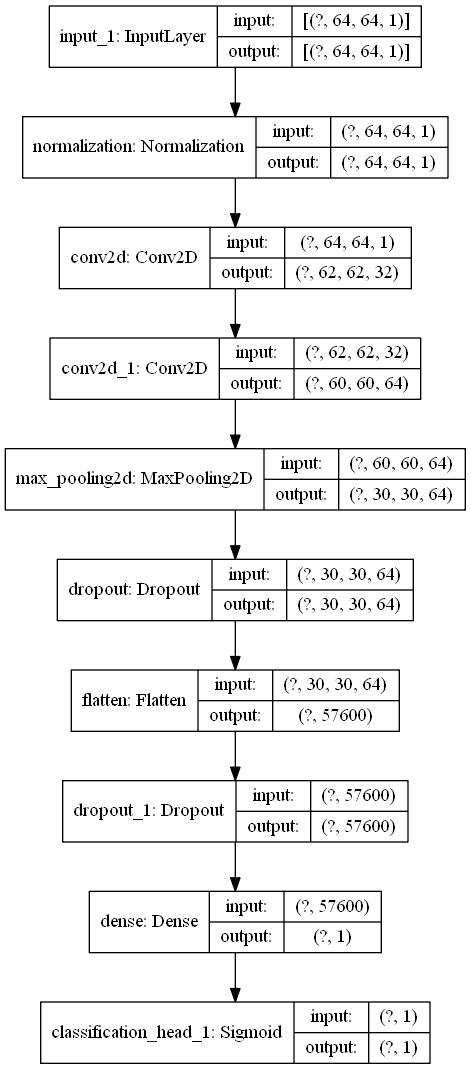
\includegraphics[width=0.7\linewidth]{img/model-samenvatting.png}
    \caption{Mogelijke lagenstructuur van een model.}
    \label{fig:layer-autokeras}
\end{figure}

\section{Resultaten}
\label{sec:results-autokeras}

\pyth{print('hello world')}

\begin{table}[ht]
    \centering
    \begin{tabular}{c c c c c c} % centered columns (4 columns)
        \hline\hline %inserts double horizontal lines
        Max aantal pogingen & Accuracy & Loss & Trainingsduur & Aantal lagen & Aantal parameters \\ [0.5ex] % inserts table
        %heading
        \hline % inserts single horizontal line
        5   & 82.74\%   & 63.83\%   & 2u    & 10    & 76.420 \\ 
        \hline %inserts single line
    \end{tabular}
    \caption{Resultaten AutoKeras}
    \label{table:autokeras-results}
\end{table}


\section{Requirements}